\section{Synthesis}
\begin{modified}
The tessellation phase extracts tiles $N\times N$ from each image. Each image is represented as a matrix of grey pixels in $\left[0,1\right]^{h \times w}$, where $h$ is the height and $w$ the width of the image. At the end of this procedure, each image is represented as a list of tiles, making it difficult to reconstruct the original image. This process, referred to as \textit{‘synthesis’}, introduces a layer of complexity that helps protect against falsification.
\end{modified}

\begin{toReview}
\noindent Falsifying an artwork under this scheme presents several challenges:
\begin{itemize}
	\item Reconstructing an image from its tiles would require an extremely complex program, as brute-force approaches are computationally infeasible due to time constraints.
	\item A forger would not only need to generate a set of plausible tiles but also ensure that these tiles can be reconstructed into a coherent image, a task far more complex than simple reconstruction.
	\item Even if the forger perturbs an image repeatedly to reduce the distance from a target author, they must still preserve the overall sense of the artwork, which the tiles alone do not guarantee.
\end{itemize}
	\noindent Furthermore, the small size of the tiles makes this process particularly robust. The tiles are large enough to capture the author’s unique handwriting traits but small enough to make manual reproduction extremely difficult. For example, with a resolution of $400$ \gls{ppi}, each pixel measures approximately $63,5\operatorname{\mathrm{\mu m}}$. Given that the pen stroke width in the dataset is around $0.4\operatorname{\mathrm{mm}}$, tiles of size $6\times6$ are sufficient to capture an entire stroke.
\end{toReview}

\begin{algorithm}[ht]
	\caption[Algorithm for tile extraction]{Algorithm for tile extraction.\\
		\begin{minipage}[t]{\linewidth}
			\textsc{INPUT}
			\begin{itemize}[noitemsep, topsep=0pt]
				\item[$\textnormal{M}$:] Matrix of gray values with shape $h\times w$
			\end{itemize}
		\end{minipage}
	}
\begin{algorithmic}[1]
\Function{TilesExtraction}{$\textnormal{M}$}
    \State $L \gets \texttt{empty list of tiles}$ \Comment{will have $(\textnormal{h} - N + 1)\times(\textnormal{w} - N+1)$ tiles}
    \For{$row \gets 0$ to $\textnormal{h} - N$, $col \gets 0$ to $\textnormal{w} - N$}
    	\State \textit{Copy tiles in coordinates $[row, row+N]\times[col,col+N]$ of matrix $\textnormal{M}$}
    	\State declare $v$ as matrix $N \times N$ \Comment{$N$ is size of tiles}
        \For{$i \gets 1$ to $N$, $j \gets 1$ to $N$}
            \State $v[i][j] \gets \textnormal{M}[row + i][col + j]$
        \EndFor
        \State call \texttt{Append}($L$, $v$) \Comment Append the tile $v$ to list $L$
    \EndFor
\EndFunction
\label{alg:SequentialTilesExtraction}
\end{algorithmic}
\end{algorithm}

\begin{figure}[ht]
    \centering
    \begin{subfigure}{0.4\linewidth}
        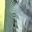
\includegraphics[width=\linewidth]{Figures/example_detail.png}
        \caption{Image detail $32 \times 32$.}
    \end{subfigure}
    \hspace{2cm}
    \begin{subfigure}{0.4\linewidth}
        
\includegraphics[width=\linewidth]{Figures/example_tiles.png}
        \caption{List of tiles $8 \times 8$.}
    \end{subfigure}
    \caption[Illustration of synthesis process]{The synthesis process convert an image in a list of its tiles.}
    \label{fig:puffer_tiles}
\end{figure}
